%==============================================================================
% BELANGRIJK - Kruisverwijzingen (relatief via \ref, geen harde nummers):
% Dit hoofdstuk verwijst naar labels in andere hoofdstukken. Zorg dat deze
% aanwezig zijn (voeg toe indien nog niet aanwezig):
%   - Hoofdstuk 1, na \chapter{...}:                        \label{ch:eerstehoofdwet}
%   - Hoofdstuk 2, na \chapter{...}:                        \label{ch:kwantum}
%     (Hoofdstuk 2 bevat reeds \label{sec:waterstofatoom},
%      \label{sec:atomaire-spectra} en \label{sec:moleculaire-beweging}.)
%   - Hoofdstuk 3 gebruikt reeds \label{ch:spontaniteit}.
%   - Hoofdstuk 5 gebruikt reeds \label{ch:niet-reagerend} (bevestigd).
%   - Hoofdstuk 9, na \chapter{...} (oppervlakte- en
%     colloïdchemie, DLVO):                                 \label{ch:oppervlakte}
%   - Hoofdstuk 11, na \chapter{...} (vaste-stofchemie en
%     kristallografie, ionische kristallen \S 11.2.3):       \label{ch:kristallografie}
%   LET OP: het voorheen aangenomen apart hoofdstuk "transportverschijnselen"
%   (\ref{ch:transport}) is niet weerhouden; diffusie is inmiddels
%   geïntegreerd in hoofdstuk 8 (\ref{ch:kinetiek}, \S~"Diffusielimitatie").
%   De verwijzing hieronder naar viscositeit/diffusie is dienovereenkomstig
%   aangepast.
% LET OP: eerdere versie van dit hoofdstuk verwees naar "Hoofdstuk 10" voor
% ionische kristallen; dat is volgens de globale inhoudsopgave hoofdstuk 11
% (Vaste-stofchemie en kristallografie). Hieronder gecorrigeerd.
% Dit bestand gebruikt de omgevingen \begin{voorbeeld}{titel}, \begin{definitie}{titel}
% en \begin{besluit}{titel} (zoals in hoofdstuk 1 en 3); enkele van deze omgevingen
% waren in de vorige versie foutief geopend als \begin{voorbeeld{titel} (ontbrekende
% sluitaccolade na de omgevingsnaam) — dit is hieronder overal gecorrigeerd.
%==============================================================================
\chapter{Intermoleculaire krachten en de vloeistoffase}
\label{ch:intermoleculair}
%==============================================================================

\section{Voorbij de covalente binding}
\label{sec:voorbij-covalent}

In hoofdstuk~\ref{ch:kwantum} zagen we hoe de kwantummechanica de oorsprong vormt van chemische bindingen en van de energie die vrijkomt of wordt opgenomen tijdens een chemische reactie. We beperkten ons daarbij tot de sterke intramoleculaire bindingen --- covalente, ionogene en metallische bindingen --- die atomen samenhouden binnen een molecule of een kristalrooster. In hoofdstuk~\ref{ch:spontaniteit} leerden we vervolgens hoe de Gibbs-vrije energie $\Delta G=\Delta H-T\Delta S$ bepaalt of een proces --- ook een fysisch proces zoals smelten, verdampen of mengen --- spontaan verloopt.

Wat in beide hoofdstukken nog ontbreekt, is een verklaring voor de \emph{enthalpie} van dergelijke fysische processen. Waarom is water bij kamertemperatuur een vloeistof terwijl methaan een gas is, hoewel beide molecules een vergelijkbare massa hebben? Waarom mengen water en ethanol wel, maar water en olie niet? Waarom bedraagt de verdampingsenthalpie van water \SI{40.7}{\kilo\joule\per\mole} terwijl die van methaan slechts \SI{8.2}{\kilo\joule\per\mole} bedraagt? Waarom kan een vloeistof worden opgewarmd boven haar kookpunt zonder te verdampen, en waarom be\"\i nvloedt een klein beetje zout het kookpunt aanzienlijk?

De verklaring ligt in de \emph{intermoleculaire krachten}: de aantrekkings- en afstotingskrachten tussen molecules, die zwakker zijn dan covalente bindingen, maar bepalend voor de fysische eigenschappen van vloeistoffen en vaste stoffen. In dit hoofdstuk ontwikkelen we een systematisch overzicht van deze krachten, kwantificeren we hun reikwijdte en sterkte, en leggen we de brug naar de thermodynamica van vloeistoffen en mengsels die in de volgende hoofdstukken wordt ontwikkeld. Waar hoofdstuk~\ref{ch:kwantum} de \emph{sterke} bindingen \emph{binnen} een molecule verklaarde, en hoofdstuk~\ref{ch:spontaniteit} het \emph{criterium} voor spontaniteit gaf, levert dit hoofdstuk de microscopische oorsprong van de energie\"en (en, via de mengentropie, gedeeltelijk ook de entropie) die in dat criterium worden ingevuld.

\section{Een classificatie van intermoleculaire krachten}

Intermoleculaire krachten worden ingedeeld naar hun fysische oorsprong. Vijf types worden onderscheiden, gerangschikt van sterk naar zwak.

\subsection{Ion--ion-interactie (Coulomb)}

Tussen twee ionen met ladingen $q_1$ en $q_2$ op afstand $r$ werkt de Coulombkracht:
\begin{equation}
V(r) = \frac{q_1 q_2}{4\pi\varepsilon_0 r}.
\end{equation}
Deze kracht is verreweg de sterkste intermoleculaire interactie en neemt slechts af als $1/r$, zodat haar reikwijdte zeer groot is. In ionische kristallen (hoofdstuk~\ref{ch:kristallografie}) is dit de dominante binding. Typische energie: \SIrange{200}{800}{\kilo\joule\per\mole}.

\subsection{Ion--dipool-interactie}
\label{sec:ion-dipool}

Wanneer een ion in de buurt komt van een polair molecule (met permanent dipoolmoment $\mu$), ontstaat een gerichte interactie. Net zoals bij de dipool--dipoolinteractie (\S~\ref{sec:keesom} hieronder) is de dipool niet star georiënteerd: thermische beweging laat hem voortdurend heroriënteren, met een voorkeur voor de aantrekkende oriëntatie. Na thermische middeling over alle oriënteringen (Boltzmann-gewogen) levert dit:
\begin{equation}
\boxed{\;V(r) = -\frac{q^2 \mu^2}{6(4\pi\varepsilon_0)^2 k_BT\, r^4}.\;}
\end{equation}
Merk op dat, net als bij de Keesom-interactie, een factor $1/T$ optreedt: bij hogere temperatuur verstoort de thermische beweging de gunstige oriëntatie sterker, zodat de netto aantrekking afneemt. (In de limiet waarin de dipool volledig vast staat ten opzichte van het ion --- bijvoorbeeld omdat het ion het dipoolmoment volledig domineert --- geldt in plaats daarvan de eenvoudigere, temperatuuronafhankelijke uitdrukking $V(r)=-q\mu/(4\pi\varepsilon_0 r^2)$; in de meeste vloeistoffen bij eindige temperatuur is de thermisch gemiddelde vorm hierboven de relevante.) Deze interactie is verantwoordelijk voor de oplosbaarheid van zouten in polaire oplosmiddelen (bv. $\mathrm{NaCl}$ in water). Typische energie: \SIrange{40}{600}{\kilo\joule\per\mole}.

\subsection{Dipool--dipool-interactie (Keesom)}
\label{sec:keesom}

Twee permanente dipolen die op een afstand $r$ van elkaar staan, ori\"enteren zich zodanig dat de aantrekkende configuratie wordt bevoordeeld. De gemiddelde interactie-energie over alle orientaties (rekening houdend met thermische beweging) is:
\begin{equation}
\boxed{\;V_{\text{Keesom}}(r) = -\frac{2\mu_1^2 \mu_2^2}{3(4\pi\varepsilon_0)^2 k_B T\, r^6}\;}
\end{equation}
Het $1/r^6$-gedrag is karakteristiek voor alle Van der Waalskrachten. De afhankelijkheid van $1/T$ verklaart waarom de intermoleculaire orientatie belangrijker wordt bij lage temperatuur. Typische energie: \SIrange{5}{25}{\kilo\joule\per\mole}.

\subsection{Dipool--ge\"induceerde dipool (Debye)}

Een permanent dipool kan een niet-polair molecule polariseren. De wisselwerkingsenergie bedraagt:
\begin{equation}
\boxed{\;V_{\text{Debye}}(r) = -\frac{\mu_1^2 \alpha_2}{(4\pi\varepsilon_0)^2 r^6}\;}
\end{equation}
waarin $\alpha_2$ de polariseerbaarheid van het niet-polaire molecule voorstelt. Deze term is onafhankelijk van temperatuur: de geïnduceerde dipool volgt de oriëntatie van de permanente dipool ogenblikkelijk en wordt niet door thermische beweging verstoord. Typische energie: \SIrange{2}{10}{\kilo\joule\per\mole}.

\subsection{London-dispersie}
\label{sec:london}

Zelfs tussen twee niet-polaire molecules bestaat een aantrekkingskracht. Deze ontstaat doordat de elektronenwolk voortdurend fluctueert, zodat op ieder ogenblik een kortstondige dipool ontstaat, die op zijn beurt een dipool in het buurmolecule induceert. De wisselwerkingsenergie bedraagt:
\begin{equation}
\boxed{\;V_{\text{London}}(r) = -\frac{3}{4}\,\frac{I_1 I_2}{I_1 + I_2}\,\frac{\alpha_1 \alpha_2}{(4\pi\varepsilon_0)^2 r^6}\;}
\end{equation}
waarin $I_1$ en $I_2$ de ionisatie-energie\"en van de beide moleculen zijn. London-dispersie is de enige aantrekkende kracht tussen niet-polaire moleculen zoals $\mathrm{N_2}$, $\mathrm{CH_4}$, edelgassen. Ze neemt toe met de polariseerbaarheid (en dus met het aantal elektronen). Typische energie: \SIrange{0.5}{5}{\kilo\joule\per\mole}, maar voor grote moleculen aanzienlijk hoger.

\begin{voorbeeld}{Kookpunten van edelgassen}
De kookpunten van de edelgassen stijgen monotoon met het atoomnummer:
\begin{itemize}
\item He: \SI{4.2}{\kelvin} (2 elektronen)
\item Ne: \SI{27.1}{\kelvin} (10)
\item Ar: \SI{87.3}{\kelvin} (18)
\item Kr: \SI{119.9}{\kelvin} (36)
\item Xe: \SI{165.0}{\kelvin} (54)
\end{itemize}
Alle edelgassen zijn volledig niet-polair, zodat enkel London-dispersie werkt. De stijgende kookpunten weerspiegelen de toenemende polariseerbaarheid van de grotere elektronenwolken. Voor Xe, met \num{54} elektronen per atoom, bedraagt de dispersie-energie reeds voldoende om de stof bij kamertemperatuur dicht bij de vloeibaarheid te houden.
\end{voorbeeld}

\subsection{Waterstofbruggen}
\label{sec:waterstofbruggen}

Een bijzonder sterke dipool--dipoolinteractie ontstaat wanneer een waterstofatoom, covalent gebonden aan een sterk elektronegatief atoom (N, O, F), in de buurt komt van een ander elektronegatief atoom met een eenzaam elektronenpaar. De \emph{waterstofbrug} is sterk gericht en kan energie\"en tot \SI{40}{\kilo\joule\per\mole} bereiken (typisch \SIrange{10}{40}{\kilo\joule\per\mole}).

\begin{voorbeeld}{Anomalie\"en van water}
Water vormt tot vier waterstofbruggen per molecule, die een ruimtelijk netwerk vormen. Hierdoor vertoont water een reeks anomalie\"en:
\begin{itemize}
\item Hoog kookpunt (\SI{100}{\celsius}) vergeleken met $\mathrm{H_2S}$ (\SI{-60}{\celsius}), hoewel $\mathrm{H_2S}$ een zwaarder molecule is.
\item Hoge verdampingsenthalpie: \SI{40.7}{\kilo\joule\per\mole} (vergeleken met \SI{8.2}{\kilo\joule\per\mole} voor methaan).
\item Maximumdichtheid bij \SI{4}{\celsius} (ijs is minder dicht dan vloeibaar water).
\item Hoge oppervlaktespanning: \SI{72}{\milli\newton\per\metre} (zie hoofdstuk~\ref{ch:oppervlakte}).
\item Hoge viscositeit, hoge warmtecapaciteit.
\end{itemize}
Alle anomalie\"en wijzen op hetzelfde: het waterstofbrugnetwerk. Zonder dit netwerk zou water bij kamertemperatuur een gas zijn, en zou leven zoals wij het kennen onmogelijk zijn.
\end{voorbeeld}

\section{Polariseerbaarheid}

De \emph{polariseerbaarheid} $\alpha$ van een molecule is de mate waarin een uitwendig elektrisch veld een dipoolmoment induceert. Een molecule in een elektrisch veld $E$ ontwikkelt een ge\"induceerd dipoolmoment:
\begin{equation}
\mu_{\text{ind}} = \alpha\,E.
\end{equation}
De polariseerbaarheid hangt af van de grootte en mobiliteit van de elektronenwolk. Grote molecules met veel elektronen, of moleculen met gedelocaliseerde $\pi$-elektronen (bv. benzeen), hebben een hoge polariseerbaarheid. De polariseerbaarheid is een kwantitatieve schakel tussen de elektronenstructuur uit hoofdstuk~\ref{ch:kwantum} en de intermoleculaire krachten.

\begin{voorbeeld}{Polariseerbaarheid en kookpunt van halogenen}
De halogenen $\mathrm{Cl_2}$, $\mathrm{Br_2}$, $\mathrm{I_2}$ hebben vergelijkbare bindingsenergie\"en maar stijgende kookpunten:
\begin{itemize}
\item $\mathrm{Cl_2}$: \SI{-34}{\celsius} (gas bij kamertemperatuur)
\item $\mathrm{Br_2}$: \SI{59}{\celsius} (vloeistof)
\item $\mathrm{I_2}$: \SI{184}{\celsius} (vast bij kamertemperatuur)
\end{itemize}
Deze trend weerspiegelt direct de stijgende polariseerbaarheid van de grotere elektronenwolken. De covalente binding binnen de molecules is vergelijkbaar, maar de intermoleculaire (dispersie-)krachten nemen sterk toe, wat leidt tot hogere kookpunten en uiteindelijk tot een vaste stof bij kamertemperatuur voor $\mathrm{I_2}$.
\end{voorbeeld}

\section{De Lennard-Jones-potentiaal}
\label{sec:lennard-jones}

De aantrekkende $1/r^6$-afhankelijkheid van de Van der Waalskrachten geldt slechts voor matig grote afstanden. Wanneer twee moleculen zeer dicht naderen, beginnen hun elektronenwolken te overlappen en treedt een sterke afstoting op (Pauli-uitsluitingsprincipe, zie hoofdstuk~\ref{ch:kwantum}). De totale interactie-energie wordt dan beschreven door een \emph{Lennard-Jones-potentiaal}:
\begin{equation}
\boxed{\;V(r) = 4\varepsilon\left[\left(\frac{\sigma}{r}\right)^{12} - \left(\frac{\sigma}{r}\right)^{6}\right]\;}
\label{eq:lennardjones}
\end{equation}
waarin:
\begin{itemize}
\item $\varepsilon$ de diepte van de potentiaalkuil (maat voor de sterkte van de attractie),
\item $\sigma$ de afstand waarop $V = 0$ (effectieve ``harde'' diameter).
\end{itemize}
Het $1/r^{12}$-gedrag is een wiskundig handige benadering van de elektronenwolk-afstoting. Het minimum van de potentiaal ligt bij $r_{\text{eq}} = 2^{1/6}\sigma \approx 1{,}122\,\sigma$.

\begin{figure}[htb]
    \centering
    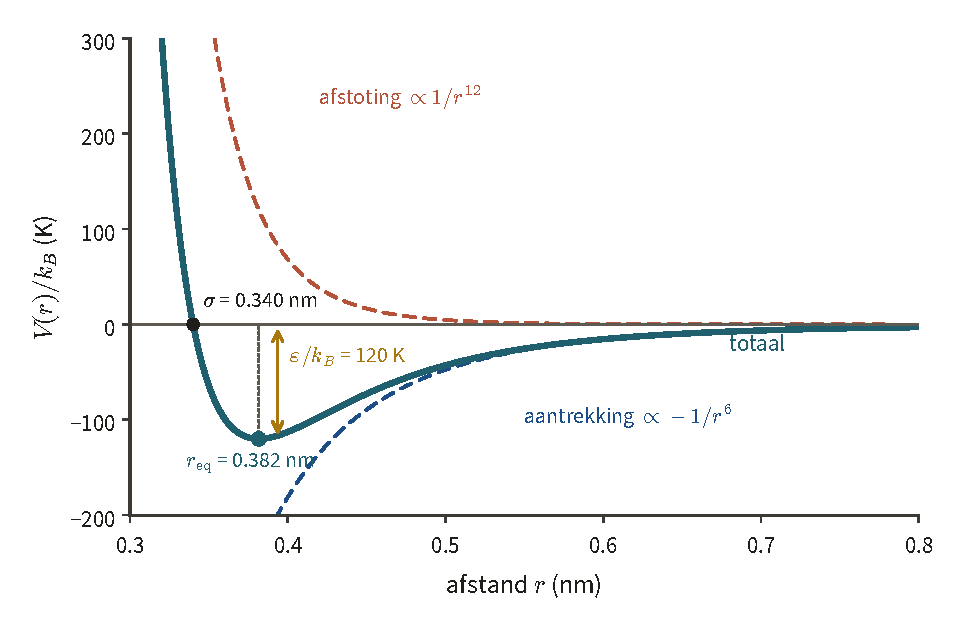
\includegraphics[width=0.7\linewidth]{Figuren/lennard_jones}
    \caption{De Lennard-Jones-potentiaal van argon ($\sigma=\SI{0.340}{\nano\metre}$, $\varepsilon/k_B=\SI{120}{\kelvin}$). De totale potentiaal (volle lijn) is de som van een steile afstoting $\propto 1/r^{12}$ en een zachtere aantrekking $\propto -1/r^6$ (stippellijnen). Het minimum ligt bij $r_{\text{eq}}=2^{1/6}\sigma$ en heeft diepte $\varepsilon$.}
    \label{fig:lennard-jones}
\end{figure}

\begin{voorbeeld}{Lennard-Jones-parameters voor argon}
\label{ex:argon-lj}
Voor argon geldt $\sigma = \SI{0.340}{\nano\metre}$ en $\varepsilon/k_B = \SI{120}{\kelvin}$ ($\varepsilon = \SI{1.65e-21}{\joule}$). De evenwichtsafstand bedraagt:
\[
r_{\text{eq}} = 2^{1/6} \cdot \SI{0.340}{\nano\metre} = \SI{0.382}{\nano\metre}.
\]
De bindingsenergie per mol bedraagt $N_A \varepsilon = \SI{994}{\joule\per\mole} \approx \SI{1.0}{\kilo\joule\per\mole}$. Dit is klein vergeleken met een covalente binding (\SI{400}{\kilo\joule\per\mole}), maar voldoende om argon bij \SI{87}{\kelvin} vloeibaar te maken. Het kookpunt blijkt inderdaad $\sim \varepsilon/k_B$, wat de fysische betekenis van de potentiaalkuil-diepte bevestigt. We gebruiken deze $\sigma$ en $\varepsilon$ verderop opnieuw (\S~\ref{sec:vdw-brug}) om de Van der Waals-parameter $a$ van argon te schatten.
\end{voorbeeld}

\section{De brug naar de vergelijking van Van der Waals}
\label{sec:vdw-brug}

In hoofdstuk~\ref{ch:eerstehoofdwet} introduceerden we de vergelijking van Van der Waals:
\begin{equation}
\left(p + \frac{a n^2}{V^2}\right)(V - nb) = nRT.
\end{equation}
De parameter $a$ corrigeert voor de intermoleculaire aantrekkingskrachten. Met behulp van de Lennard-Jones-potentiaal kan deze parameter fysisch worden ge\"interpreteerd en, in tegenstelling tot een louter evenredigheidsargument, ook effectief worden berekend.

Beschouw \'e\'en molecule, omringd door een gemiddelde, uniforme dichtheid van andere moleculen. Het aantal buurmoleculen in een dunne bolschil met straal $r$ en dikte $\dd{r}$ bedraagt $4\pi r^2\,\dd{r}$ maal de getalsdichtheid. De gemiddelde aantrekkingsenergie van \'e\'en molecule met al zijn buren wordt dan bekomen door de attractieve term van de Lennard-Jonespotentiaal, $V_{\text{attr}}(r) = -4\varepsilon(\sigma/r)^6$, te integreren over alle afstanden vanaf het punt waar de moleculen elkaar raken ($r=\sigma$) tot oneindig ver:
\begin{equation}
\overline{V}_{\text{attr}} = \int_{\sigma}^{\infty} 4\pi r^2\,V_{\text{attr}}(r)\,\dd{r} = -16\pi\varepsilon\sigma^6\int_{\sigma}^{\infty}\frac{\dd{r}}{r^4} = -16\pi\varepsilon\sigma^6\left[-\frac{1}{3r^3}\right]_{\sigma}^{\infty} = -\frac{16\pi}{3}\varepsilon\sigma^3.
\end{equation}
Omdat elk paar moleculen bij deze telling tweemaal wordt meegerekend (net zoals bij de afleiding van het co-volume $b$ in hoofdstuk~\ref{ch:eerstehoofdwet}, \S~\ref{sec:vdw-afleiding}), bedraagt de effectieve aantrekkingsenergie per mol de helft hiervan, vermenigvuldigd met het aantal Avogadro-paren:
\begin{equation}
\boxed{
a = -\frac{N_A^2}{2}\,\overline{V}_{\text{attr}} = \frac{8\pi}{3}N_A^2\,\varepsilon\sigma^3.
}
\label{eq:a-vdw-lj}
\end{equation}
De parameter $a$ is dus evenredig met het volume van de molecule ($\sigma^3$) en de diepte van de interactiekuil ($\varepsilon$), en vergelijking~\eqref{eq:a-vdw-lj} geeft bovendien de exacte evenredigheidsconstante binnen dit vereenvoudigde model. Hiermee krijgt de $a$-parameter uit hoofdstuk~\ref{ch:eerstehoofdwet} een microscopische fundering.

\begin{voorbeeld}{De Van der Waals-parameter $a$ van argon, geschat uit de Lennard-Jonespotentiaal}
Met de waarden $\sigma=\SI{0.340}{\nano\metre}$ en $\varepsilon=\SI{1.65e-21}{\joule}$ voor argon (voorbeeld~\ref{ex:argon-lj}) levert vergelijking~\eqref{eq:a-vdw-lj}:
\[
a = \frac{8\pi}{3}(6.022\times10^{23})^2(1.65\times10^{-21}\,\mathrm{J})(0.340\times10^{-9}\,\mathrm{m})^3 \approx \SI{0.197}{\pascal\,\metre^6\per\mole\squared}.
\]
De experimentele Van der Waals-parameter van argon bedraagt $a_{\text{Ar}}\approx\SI{0.1355}{\pascal\,\metre^6\per\mole\squared}$ (hoofdstuk~\ref{ch:eerstehoofdwet}, tabel met stofconstanten). Onze eenvoudige schatting zit dus binnen een factor anderhalf van de experimentele waarde --- een opmerkelijk goede overeenstemming voor een model dat de moleculaire dichtheid rond een molecule als uniform veronderstelt (dat wil zeggen: het verwaarloost dat buurmoleculen elkaar afschermen, wat in werkelijkheid door de paarcorrelatiefunctie $g(r)$ wordt beschreven). Dit bevestigt dat de Lennard-Jonesparameters $\varepsilon$ en $\sigma$, oorspronkelijk ingevoerd om spectroscopische en botsingsdata te beschrijven, en de macroscopische Van der Waals-parameter $a$, oorspronkelijk ingevoerd om afwijkingen van de ideale gaswet te beschrijven, twee kwantitatief consistente beschrijvingen zijn van dezelfde onderliggende intermoleculaire aantrekking.
\end{voorbeeld}

\section{Verdampingsenthalpie als maat voor cohesie}
\label{sec:verdampingsenthalpie}

De verdampingsenthalpie $\Delta H_{\text{vap}}$ van een zuivere vloeistof is de energie die nodig is om een molecule uit de vloeistoffase naar de gasfase te brengen, en dus om alle intermoleculaire interacties met zijn buren te verbreken. $\Delta H_{\text{vap}}$ is daarmee een directe experimentele maat voor de totale sterkte van de intermoleculaire krachten.

\begin{table}[h]
\centering
\begin{tabular}{lccc}
\toprule
Stof & $\Delta H_{\text{vap}}$ (\si{\kilo\joule\per\mole}) & $T_b$ & Dominante kracht \\
\midrule
He & 0{,}08 & \SI{4.2}{\kelvin} & Dispersie (zwak) \\
$\mathrm{N_2}$ & 5{,}6 & \SI{77.4}{\kelvin} & Dispersie \\
$\mathrm{CH_4}$ & 8{,}2 & \SI{111.7}{\kelvin} & Dispersie \\
$\mathrm{CHCl_3}$ & 29{,}4 & \SI{334.3}{\kelvin} & Dipool--dipool + dispersie \\
$\mathrm{NH_3}$ & 23{,}4 & \SI{239.8}{\kelvin} & Waterstofbrug (zwakker dan water) \\
$\mathrm{H_2O}$ & 40{,}7 & \SI{373.15}{\kelvin} & Waterstofbrug \\
Ethanol & 38{,}6 & \SI{351.55}{\kelvin} & Waterstofbrug \\
$\mathrm{NaCl}$ (sublimatie) & 211 & sublimeert & Ion--ion \\
\bottomrule
\end{tabular}
\caption{Verdampingsenthalpie\"en en normale kookpunten $T_b$ (bij \SI{1}{\bar}).}
\label{tab:verdampingsenthalpie}
\end{table}

De tabel toont duidelijk de hi\"erarchie: dispersie $<$ dipool--dipool $<$ waterstofbrug $<$ ion--ion. Zij beantwoordt bovendien meteen \'e\'en van de openingsvragen van dit hoofdstuk (\S~\ref{sec:voorbij-covalent}): methaan en stikstof, met een vergelijkbare molaire massa als water, bezitten enkel zwakke dispersiekrachten en koken daardoor al ver onder kamertemperatuur, terwijl water dankzij zijn waterstofbrugnetwerk pas bij \SI{373.15}{\kelvin} kookt. Voor de ingenieur is $\Delta H_{\text{vap}}$ een directe indicator voor het energieverbruik van een destillatieproces --- water en ethanol vereisen aanzienlijk meer energie dan koolwaterstoffen.

\subsection{De regel van Trouton}
\label{sec:trouton}

Tabel~\ref{tab:verdampingsenthalpie} bevat zowel $\Delta H_{\text{vap}}$ als het normale kookpunt $T_b$: de temperatuur waarbij, per definitie, de vloeistof- en dampfase bij \SI{1}{\bar} in evenwicht zijn. Uit hoofdstuk~\ref{ch:spontaniteit} (\S~\ref{sec:entropie-faseovergangen}) weten we dat voor elke reversibele faseovergang bij constante druk geldt $\Delta S_{\text{trans}}=\Delta H_{\text{trans}}/T_{\text{trans}}$. Toegepast op verdamping:
\begin{equation}
\Delta S_{\text{vap}} = \frac{\Delta H_{\text{vap}}}{T_b}.
\end{equation}
De empirische \emph{regel van Trouton} stelt dat deze verdampingsentropie voor de meeste ``normale'' vloeistoffen --- dat wil zeggen vloeistoffen zonder sterke, gerichte intermoleculaire interacties zoals waterstofbruggen --- ongeveer dezelfde waarde aanneemt, typisch $\Delta S_{\text{vap}}\approx\SIrange{85}{88}{\joule\per\mole\per\kelvin}$. De fysische reden is intuïtief: bij het koken wint elke vloeistof, ongeacht haar chemische aard, ongeveer dezelfde \emph{relatieve} toename in bewegingsvrijheid (van een gecondenseerde naar een verdunde gasfase), zodat de toename in het aantal toegankelijke microtoestanden (\S~\ref{sec:waarschijnlijkheid-entropie} in hoofdstuk~\ref{ch:spontaniteit}) voor de meeste vloeistoffen vergelijkbaar is.

\begin{voorbeeld}{Trouton's regel getoetst aan tabel~\ref{tab:verdampingsenthalpie}}
We berekenen $\Delta S_{\text{vap}}=\Delta H_{\text{vap}}/T_b$ voor elke stof uit tabel~\ref{tab:verdampingsenthalpie}:
\begin{center}
\begin{tabular}{lc}
\toprule
Stof & $\Delta S_{\text{vap}}$ (\si{\joule\per\mole\per\kelvin}) \\
\midrule
$\mathrm{N_2}$ (dispersie) & $5600/77.4 = 72.4$ \\
$\mathrm{CH_4}$ (dispersie) & $8200/111.7 = 73.4$ \\
$\mathrm{CHCl_3}$ (dipool--dipool) & $29400/334.3 = 87.9$ \\
$\mathrm{NH_3}$ (zwakke waterstofbrug) & $23400/239.8 = 97.6$ \\
$\mathrm{H_2O}$ (waterstofbrug) & $40700/373.15 = 109.1$ \\
Ethanol (waterstofbrug) & $38600/351.55 = 109.8$ \\
\bottomrule
\end{tabular}
\end{center}
Het patroon is opmerkelijk consistent: chloroform, dat enkel dipool--dipool- en dispersiekrachten bezit, voldoet vrijwel exact aan de regel van Trouton ($\approx\SI{88}{\joule\per\mole\per\kelvin}$). Stikstof en methaan liggen er iets onder (een bekende afwijking voor kleine, quasi-boldeeltjes met weinig interne vrijheidsgraden, zie hoofdstuk~\ref{ch:kwantum}, \S~\ref{sec:moleculaire-beweging}). Ammoniak, water en ethanol wijken daarentegen sterk en systematisch \emph{naar boven} af: hun waterstofbrugnetwerk (\S~\ref{sec:waterstofbruggen}) moet bij het verdampen worden opgebroken, wat een extra, geordend-naar-ongeordend effect toevoegt bovenop de gewone toename in bewegingsvrijheid. Merk op dat de waarde voor water, $\SI{109.1}{\joule\per\mole\per\kelvin}$, overeenkomt met de waarde $\Delta S_{\text{vap}}\approx\SI{109}{\joule\per\mole\per\kelvin}$ die reeds in hoofdstuk~\ref{ch:spontaniteit} werd berekend. Trouton's regel levert een ingenieur zo een snelle, eerste-orde consistentiecontrole: een sterke afwijking van $\approx\SI{85}{\joule\per\mole\per\kelvin}$ is een directe indicatie van gerichte intermoleculaire interacties (waterstofbruggen) die in een proces- of destillatieontwerp niet over het hoofd mogen worden gezien.
\end{voorbeeld}

\section{Mengsels: regelmatige oplossingen en de Hildebrand-parameter}

Wanneer twee vloeistoffen mengen, worden intermoleculaire interacties verbroken en nieuwe gevormd. De mengenthalpie is de nettobalans hiervan. Voor \emph{regelmatige oplossingen} (geen waterstofbruggen, geen sterke dipoolinteracties) ontwikkelde Hildebrand een kwantitatieve theorie.

\subsection{De Hildebrand-oplosbaarheidsparameter}
\label{sec:hildebrand}

De \emph{Hildebrand-parameter} $\delta$ is gedefinieerd als:
\begin{equation}
\boxed{\;\delta = \sqrt{\frac{\Delta E_{\text{vap}}}{V_m}}\;}
\end{equation}
waarin $\Delta E_{\text{vap}} = \Delta H_{\text{vap}} - RT$ de molaire verdampingsenergie (energie, niet enthalpie) en $V_m$ het molaire volume zijn. De eenheid is \si{\joule\per\centi\metre\cubed} of equivalent \si{\mega\pascal^{1/2}}.

De mengenthalpie voor twee vloeistoffen met gelijke volumes wordt benaderd door:
\begin{equation}
\Delta H_{\text{meng}} \approx V\,(\delta_1 - \delta_2)^2\,\phi_1\,\phi_2,
\end{equation}
waarin $\phi_i$ de volumefracties zijn. \emph{Gelijksoortige $\delta$-waarden leiden tot mengbaarheid}; sterk verschillende waarden leiden tot demixing --- via het spontaniteitscriterium $\Delta G_{\text{meng}}=\Delta H_{\text{meng}}-T\Delta S_{\text{meng}}$ uit hoofdstuk~\ref{ch:spontaniteit}: wanneer $\Delta H_{\text{meng}}$ voldoende groot en positief is, kan het de (steeds positieve, maar begrensde) mengentropiebijdrage $-T\Delta S_{\text{meng}}$ overtreffen, zodat $\Delta G_{\text{meng}}>0$ en de vloeistoffen zich spontaan ontmengen.

\begin{voorbeeld}{Water en hexaan}
De Hildebrand-parameters bedragen:
\begin{itemize}
\item Water: $\delta = \SI{47.9}{\mega\pascal^{1/2}}$ (sterk waterstofbruggend)
\item $n$-Hexaan: $\delta = \SI{14.9}{\mega\pascal^{1/2}}$ (niet-polair koolwaterstof)
\end{itemize}
Het verschil is groot, waardoor $\Delta H_{\text{meng}}$ zeer positief is. De Gibbs-energie van mengen (hoofdstuk~\ref{ch:niet-reagerend}, \S~\ref{sec:thermodynamica-mengsels}) wordt dan positief, en de vloeistoffen mengen niet. Dit verklaart, kwantitatief, waarom olie en water zich splitsen --- exact de vraag die in \S~\ref{sec:voorbij-covalent} werd gesteld.

Voor twee koolwaterstoffen, bv. hexaan ($\delta = \SI{14.9}{\mega\pascal^{1/2}}$) en heptaan ($\delta = \SI{15.2}{\mega\pascal^{1/2}}$), is het verschil klein en mengen de vloeistoffen volledig. In de chromatografie en de verfindustrie wordt de Hildebrand-parameter gebruikt om compatibele oplosmiddelen te selecteren.
\end{voorbeeld}

\subsection{Beperkingen}

De Hildebrand-theorie werkt goed voor niet-polaire of zwak polaire mengsels zonder specifieke interacties. Voor systemen met waterstofbruggen (water, alcoholen) of sterke dipoolinteracties bestaat geen enkelvoudige theorie die zonder meer bruikbaar is; de Hansen-parameters, die $\delta$ opsplitsen in dispersie-, dipool- en waterstofbrug-bijdragen, bieden een verbetering.

\section{Sterkte en reikwijdte}
\label{sec:sterkte-reikwijdte}

Een belangrijk onderscheid tussen de intermoleculaire krachten is hun \emph{reikwijdte}:

\begin{itemize}
\item \textbf{Ion--ion}: $V \propto 1/r$ --- lange reikwijdte, orde van meerdere nanometer.
\item \textbf{Ion--dipool}: $V \propto 1/r^4$ --- matige reikwijdte.
\item \textbf{Van der Waals} (Keesom, Debye, London): $V \propto 1/r^6$ --- korte reikwijdte, enkel significant binnen \SI{1}{\nano\metre}.
\item \textbf{Waterstofbrug}: sterk gericht, typisch \SIrange{0.18}{0.25}{\nano\metre}.
\end{itemize}

\begin{figure}[htb]
    \centering
    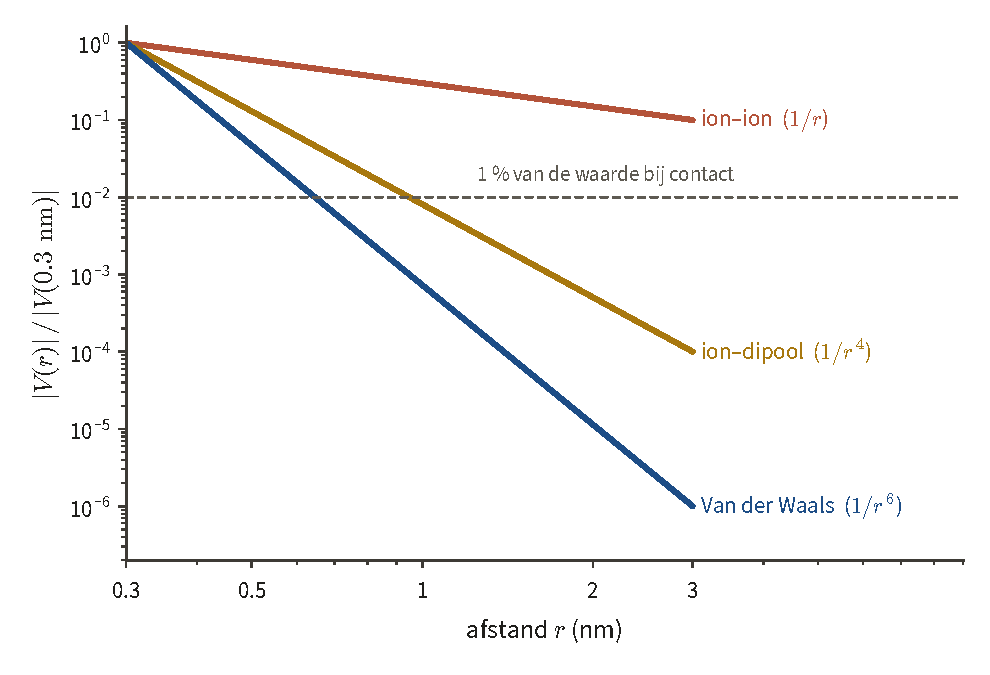
\includegraphics[width=0.7\linewidth]{Figuren/reikwijdte}
    \caption{Relatieve sterkte van de interactie-energie $|V(r)|$ als functie van de afstand, op een logaritmische schaal en genormaliseerd op $r = \SI{0.3}{\nano\metre}$. De Coulombinteractie tussen ionen ($1/r$) reikt veel verder dan de ion--dipoolinteractie ($1/r^4$) en de Van der Waalskrachten ($1/r^6$). Bij een verdubbeling van de afstand daalt een Van der Waalsinteractie met een factor 64.}
    \label{fig:reikwijdte}
\end{figure}

Dit onderscheid is belangrijk voor de collo\"idchemie (hoofdstuk~\ref{ch:oppervlakte}): bij de DLVO-theorie worden lange-reikwijdte elektrostatische afstoting (van geladen oppervlakken) vergeleken met korte-reikwijdte Van der Waals-aantrekking.

\section{Kwantitatieve vergelijking van de krachten}

De volgende tabel geeft een orde-grootte-overzicht van alle behandelde interacties:

\begin{table}[h]
\centering
\begin{tabular}{lcc}
\toprule
Type & Energie (\si{\kilo\joule\per\mole}) & Afhankelijkheid \\
\midrule
Covalente binding & 200--800 & Complex \\
Ion--ion & 200--800 & $1/r$ \\
Ion--dipool & 40--600 & $1/r^4$, $1/T$ \\
Waterstofbrug & 10--40 & Gericht, \SI{0.2}{\nano\metre} \\
Dipool--dipool (Keesom) & 5--25 & $1/r^6$, $1/T$ \\
Dipool--ge\"ind. (Debye) & 2--10 & $1/r^6$ \\
Dispersie (London) & 0{,}5--10 & $1/r^6$ \\
\bottomrule
\end{tabular}
\caption{Ordes van grootte van intermoleculaire krachten.}
\end{table}

Een opvallende observatie: alle Van der Waalskrachten (Keesom, Debye, London) delen dezelfde $1/r^6$-afhankelijkheid. Dit is geen toeval: alle drie zijn ze zwakke storingen van de elektronenstructuur, en dezelfde wiskundige structuur geldt. Merk verder op dat de energiebereiken van de covalente binding en de ion--ioninteractie elkaar volledig overlappen: het onderscheid tussen ``intramoleculair'' en ``intermoleculair'' is dus niet in de eerste plaats een kwestie van energieschaal, maar van de aard van de interactie (gedeelde elektronenparen versus elektrostatische aantrekking tussen afgeronde ladingen, hoofdstuk~\ref{ch:kwantum}).

\section{Intermoleculaire krachten aan het werk}
\label{sec:im-toepassingen}

Intermoleculaire krachten zijn zwak in vergelijking met chemische bindingen, maar ze werken overal en altijd. In deze paragraaf bekijken we een reeks situaties uit het dagelijks leven en de industrie waarin ze de doorslag geven. Telkens stellen we dezelfde vraag: \emph{welke kracht domineert, en wat volgt daaruit?}

\begin{toepassing}{Water koken: veel energie, en soms een verrassing}
Om water te verdampen moeten alle waterstofbruggen van een molecule met zijn buren verbroken worden. Daarom is de verdampingsenthalpie van water per kilogram uitzonderlijk hoog: \SI{2257}{\kilo\joule\per\kilo\gram}, tegenover \SI{838}{} voor ethanol en \SI{335}{\kilo\joule\per\kilo\gram} voor hexaan. Dat maakt stoom de ideale warmtedrager in de industrie: een kilogram condenserende stoom levert veel warmte bij een constante temperatuur. Om dezelfde reden is een koeltoren zo effici\"ent: verdampt \SI{1}{\percent} van het koelwater, dan koelt de rest ongeveer \SI{5}{\kelvin} af.

De sterke cohesie heeft ook een keerzijde. Een dampbel kan pas groeien als ze groot genoeg is om de oppervlaktespanning te overwinnen. In een zeer gladde, schone kom (bv.\ een glas water in de microgolfoven) ontbreken de kleine oneffenheden of luchtbelletjes waarop bellen kunnen ontstaan. Het water kan dan enkele graden boven \SI{100}{\celsius} komen zonder te koken, en bij de minste verstoring explosief opkoken. In het labo voorkom je dat met kookstenen; in een verdamper met een ruw oppervlak of een kleine gasstroom.
\end{toepassing}

\begin{toepassing}{Lijmen en kleefband: contact is alles}
Een lijm of een kleefband hecht vooral via Van der Waalskrachten en, als de oppervlakken polair zijn, via waterstofbruggen. Hoe sterk kan dat zijn? Voor twee vlakke oppervlakken op afstand $D$ geeft de theorie een aantrekking per oppervlakte
\begin{equation}
\frac{F}{A} = \frac{A_\mathrm{H}}{6\pi D^3},
\label{eq:hamaker}
\end{equation}
met $A_\mathrm{H} \approx \SI{1e-19}{\joule}$ de \emph{Hamakerconstante}. Bij moleculair contact ($D \approx \SI{0.4}{\nano\metre}$) is dat
\[
\frac{F}{A} = \frac{10^{-19}}{6\pi(0.4\times10^{-9})^3} \approx \SI{8e7}{\pascal} = \SI{800}{\bar}.
\]
Twee perfect vlakke oppervlakken zouden dus enorm sterk aan elkaar kleven. In de praktijk raken twee vaste stoffen elkaar maar op enkele toppen van hun ruwheid; elders is $D$ honderden keren groter, en door de $1/D^3$-afhankelijkheid valt de kracht weg. Daarom is een lijm altijd \emph{vloeibaar} wanneer hij wordt aangebracht: hij vloeit in alle oneffenheden en maakt zo overal moleculair contact. Pas daarna hardt hij uit.

De gekko gebruikt hetzelfde principe zonder lijm. Zijn tenen dragen miljoenen fijne haartjes die zich elk afzonderlijk aan de ruwheid van een muur aanpassen. De gemeten hechting, ongeveer \SI{10}{\newton\per\square\centi\metre}, is duizendmaal minder dan de theoretische waarde, maar ruim voldoende om het dier aan \'e\'en poot te laten hangen.

Waarom kleeft bijna niets aan polyetheen of teflon? Hun oppervlak heeft enkel zwakke dispersiekrachten en geen polaire groepen (lage \emph{oppervlakte-energie}: \SI{20}{} tot \SI{33}{\milli\joule\per\square\metre}, tegenover \SI{72}{} voor water en ruim boven \SI{100}{} voor glas of metaal). Een lijm bevochtigt zo'n oppervlak slecht. Industrieel behandelt men kunststof daarom eerst met een corona- of plasmabehandeling, die polaire groepen (\ce{-OH}, \ce{-COOH}) op het oppervlak aanbrengt.
\end{toepassing}

\begin{toepassing}{Coatings: waterafstotend, krasvast of vuilafstotend}
Een coating moet aan de ondergrond hechten, maar haar buitenkant moet vaak net \emph{niet} kleven. Een waterafstotende coating (teflon, siliconen, fluorhoudende impregneermiddelen voor textiel) heeft aan de buitenkant enkel \ce{-CF3}- of \ce{-CH3}-groepen. Water vormt er geen waterstofbruggen mee en trekt zich samen tot druppels. Fluor is daarbij bijzonder effectief: het is klein en zeer weinig polariseerbaar, zodat zelfs de dispersiekrachten zwak zijn.

Bij het formuleren van een verf kies je het oplosmiddel met de Hildebrandparameter uit \S~\ref{sec:hildebrand}: het oplosmiddel moet het bindmiddel (de polymeerhars) goed oplossen, dus een vergelijkbare $\delta$ hebben, en daarna snel genoeg verdampen. Dezelfde redenering verklaart waarom aceton een verflaag of piepschuim aantast, en water niet.
\end{toepassing}

\begin{toepassing}{Adsorptie: moleculen vasthouden op een oppervlak}
Actieve kool heeft een inwendig oppervlak van \SIrange{500}{1500}{\square\metre\per\gram}: \'e\'en theelepel heeft het oppervlak van een voetbalveld. Organische moleculen blijven er via dispersiekrachten aan hangen (\emph{fysisorptie}, typisch \SIrange{5}{40}{\kilo\joule\per\mole}). Grote, goed polariseerbare moleculen (oplosmiddeldampen, geurstoffen, chloor uit leidingwater) worden het sterkst vastgehouden; kleine, weinig polariseerbare gassen zoals \ce{N2} en \ce{O2} nauwelijks. Daarom werkt een actief-koolfilter in een dampkap of een gasmasker.

Zeolieten zijn kristallijne alumino-silicaten met pori\"en van moleculaire afmetingen en geladen kationen (\ce{Na+}, \ce{Ca^2+}) in hun wanden. Watermoleculen binden er via ion--dipoolinteracties, met een adsorptie-enthalpie die hoger ligt dan de condensatie-enthalpie van water. Zeolieten drogen gassen en oplosmiddelen daardoor tot extreem lage watergehaltes. Zuurstofconcentratoren gebruiken een zeoliet die \ce{N2} sterker bindt dan \ce{O2}: het quadrupoolmoment van \ce{N2} is groter en interageert met de kationen. Adsorptie komt uitgebreid terug in hoofdstuk~\ref{ch:oppervlakte}.
\end{toepassing}

\begin{toepassing}{Nylon versus polyetheen}
Polyetheen (PE) en nylon-6,6 zijn beide lange ketens, maar hun eigenschappen verschillen sterk. Tussen PE-ketens werken enkel dispersiekrachten; HDPE smelt rond \SI{130}{\celsius}. In nylon vormen de amidegroepen (\ce{-CO-NH-}) waterstofbruggen tussen naburige ketens; nylon-6,6 smelt pas bij \SI{265}{\celsius}, is stijver en sterker. Kevlar gaat nog verder: zijn starre ketens liggen perfect geordend naast elkaar met een waterstofbrug om de paar atomen. Per gewicht is een Kevlarvezel vijf keer sterker dan staal.

De keerzijde: dezelfde amidegroepen trekken water aan. Nylon neemt enkele procent vocht op, zwelt en wordt zachter. Bij het spuitgieten moet nylongranulaat daarom eerst gedroogd worden.
\end{toepassing}

\begin{toepassing}{Smeermiddelen}
Een smeerolie bestaat uit lange koolwaterstofketens. De dispersiekrachten tussen de ketens bepalen de viscositeit: langere ketens geven meer contactpunten en een dikkere olie. Bij hogere temperatuur bewegen de ketens sneller en daalt de viscositeit sterk; additieven (lange polymeren die bij hoge temperatuur ontrollen) beperken dat effect. Vaste smeermiddelen zoals grafiet en \ce{MoS2} hebben een gelaagde structuur: binnen een laag sterke covalente bindingen, tussen de lagen enkel zwakke Van der Waalskrachten. De lagen schuiven daardoor gemakkelijk over elkaar.
\end{toepassing}

\begin{toepassing}{Koelmiddelen en luchtscheiding}
Een koelmiddel moet verdampen bij een lage temperatuur (zwakke intermoleculaire krachten) en daarbij toch veel warmte opnemen (voldoende sterke krachten). Ammoniak, met waterstofbruggen, kookt bij \SI{-33}{\celsius} en neemt \SI{1370}{\kilo\joule\per\kilo\gram} op; het fluorhoudende R-134a kookt bij \SI{-26}{\celsius} maar neemt slechts \SI{217}{\kilo\joule\per\kilo\gram} op. Ammoniak is daarom het koelmiddel van grote industri\"ele installaties (koelhuizen, brouwerijen), ondanks zijn giftigheid.

Bij de cryogene luchtscheiding worden stikstof (kookpunt \SI{77.4}{\kelvin}), argon (\SI{87.3}{\kelvin}) en zuurstof (\SI{90.2}{\kelvin}) door destillatie gescheiden. Deze moleculen hebben enkel dispersiekrachten van vergelijkbare sterkte; de kookpunten liggen daardoor dicht bij elkaar en de kolommen zijn hoog, met tientallen schotels.
\end{toepassing}

\begin{toepassing}{DNA en geneesmiddelen}
De twee strengen van DNA worden samengehouden door waterstofbruggen tussen de basen: twee tussen A en T, drie tussen G en C. Elke brug is zwak, maar met duizenden achter elkaar is de dubbele helix stabiel. Bij verhitting tot ongeveer \SI{95}{\celsius} breken ze en gaan de strengen uit elkaar; de PCR-techniek benut dat. Een geneesmiddel werkt op dezelfde manier: het past in de holte van een eiwit en wordt daar vastgehouden door een combinatie van waterstofbruggen, ionische interacties en dispersiekrachten. Een kleine wijziging van \'e\'en groep kan de binding honderd keer sterker of zwakker maken.
\end{toepassing}

\section{Samenvatting en reflectie}

\begin{samenvatting}{Intermoleculaire krachten}
\begin{itemize}
\item Intermoleculaire krachten zijn van elektrostatische oorsprong. Van sterk naar zwak: ion--ion, ion--dipool, waterstofbrug, dipool--dipool (Keesom), dipool--ge\"induceerde dipool (Debye) en dispersie (London).
\item Dispersiekrachten werken tussen alle moleculen en groeien met de polariseerbaarheid, dus met de grootte van de elektronenwolk. Bij grote moleculen domineren ze vaak.
\item De Lennard-Jonespotentiaal combineert afstoting ($1/r^{12}$) en aantrekking ($1/r^6$); de parameters $\varepsilon$ en $\sigma$ hangen samen met de Van der Waalsconstanten $a$ en $b$.
\item De verdampingsenthalpie is een maat voor de cohesie. Volgens de regel van Trouton is $\Delta S_\mathrm{vap} \approx \SI{85}{\joule\per\mole\per\kelvin}$; vloeistoffen met waterstofbruggen wijken naar boven af.
\item De Hildebrandparameter $\delta = \sqrt{\Delta E_\mathrm{vap}/V_\mathrm{m}}$ voorspelt de mengbaarheid: gelijkaardige $\delta$ mengt.
\item Toepassingen: koken en stoom als warmtedrager, lijmen (contact is alles, $F/A \propto 1/D^3$), coatings, adsorptie, polymeren, smeermiddelen, koelmiddelen en biomoleculen.
\end{itemize}
\end{samenvatting}

\begin{reflectie}{Intermoleculaire krachten}
\begin{enumerate}
\item Methaan en water hebben bijna dezelfde molaire massa. Waarom is het ene een gas en het andere een vloeistof bij kamertemperatuur?
\item Waarom stijgt het kookpunt van de alkanen met de ketenlengte, terwijl de moleculen niet polair zijn?
\item Een lijm hecht goed op glas, maar niet op een plastic boterpot. Verklaar, en geef een industri\"ele oplossing.
\item Waarom moet een lijm vloeibaar zijn wanneer je hem aanbrengt?
\item Waarom houdt actieve kool tolueendamp goed vast en stikstof nauwelijks?
\item Nylon en polyetheen zijn beide lange polymeerketens. Waarom smelt nylon bij een veel hogere temperatuur, en waarom moet het gedroogd worden voor verwerking?
\item Welke eigenschappen zoek je in een goed koelmiddel, en hoe hangen die samen met de intermoleculaire krachten?
\end{enumerate}
\end{reflectie}

Intermoleculaire krachten blijven in de volgende hoofdstukken op de achtergrond aanwezig: in de afwijkingen van de wet van Raoult en de activiteitsco\"effici\"enten (hoofdstuk~\ref{ch:niet-reagerend}) en in de adsorptie en oppervlaktespanning (hoofdstuk~\ref{ch:oppervlakte}).

\newpage
\section{Oefeningen}

% Oefeningen bij dit hoofdstuk (ingevoegd achteraan het hoofdstuk met \input).
% Een oefening:  \begin{oefening}[titel] ... \end{oefening}   (boek en website)
% De oplossing:  \begin{oplossing} ... \end{oplossing}       (enkel website, dichtgeklapt)

Constanten: $R = \SI{8.314}{\joule\per\mole\per\kelvin}$, $k_B = \SI{1.381e-23}{\joule\per\kelvin}$, $N_A = \SI{6.022e23}{\per\mole}$, $4\pi\varepsilon_0 = \SI{1.113e-10}{\coulomb\squared\per\joule\per\metre}$.

\begin{oefening}[Kookpunten van een homologe reeks]
De kookpunten van de \(n\)-alkanen bij \(1\,\mathrm{bar}\) zijn:

\begin{center}
\begin{tabular}{lllllll}
\toprule
Alkaan & \(\mathrm{CH_4}\) & \(\mathrm{C_2H_6}\) & \(\mathrm{C_3H_8}\) & \(\mathrm{C_4H_{10}}\) & \(\mathrm{C_5H_{12}}\) & \(\mathrm{C_6H_{14}}\) \\
\midrule
\(T_b\) (°C) & \(-162\) & \(-89\) & \(-42\) & \(0\) & \(36\) & \(69\) \\
\bottomrule
\end{tabular}
\end{center}

\begin{enumerate}
\item[(a)]
  Verklaar de trend vanuit intermoleculaire krachten. Welke kracht is dominant?
\item[(b)]
  Waarom stijgt het kookpunt minder snel naarmate de keten langer wordt?
\item[(c)]
  Voorspel het kookpunt van \(n\)-octaan (\(\mathrm{C_8H_{18}}\)).
\end{enumerate}
\end{oefening}
\begin{oplossing}
\textbf{Resultaat:} (a) \textbf{London-dispersie}. (c) \(T_b\)(octaan) \ensuremath{\approx{}} \textbf{125 °C} (experimenteel 126 °C).

\textbf{(a)} Alkanen zijn apolair: enkel London-dispersie werkt. Elke extra \(\mathrm{CH_2}\)-groep voegt elektronen toe, waardoor de polariseerbaarheid en het contactoppervlak tussen de ketens toenemen. De dispersie-energie per molecule stijgt en er is meer warmte nodig om de moleculen uit de vloeistof te halen.

\textbf{(b)} Elke \(\mathrm{CH_2}\)-groep voegt een ongeveer constant bedrag toe aan \(\Delta H_{\text{vap}}\) (ongeveer \(4\)--\(5\,\mathrm{kJ/mol}\)). Volgens Trouton is \(T_b \approx \Delta H_{\text{vap}}/\Delta S_{\text{vap}}\); in absolute temperatuur is een zelfde stijging van \(\Delta H_{\text{vap}}\) relatief steeds kleiner. Bovendien kunnen lange ketens opkrullen, waardoor niet elke extra groep volledig in contact komt met de buren.

\textbf{(c)} De stijging per koolstofatoom daalt van \(73\) naar \(33\,^\circ\mathrm{C}\); extrapolatie (ongeveer \(+30\) en \(+28\,^\circ\mathrm{C}\) voor \(\mathrm{C_7}\) en \(\mathrm{C_8}\)) geeft \(T_b \approx 125\,^\circ\mathrm{C}\). De experimentele waarde is \(126\,^\circ\mathrm{C}\). Dit is precies waarom men ruwe olie in een destillatiekolom kan scheiden in fracties: gas, benzine, kerosine, diesel.
\end{oplossing}

\begin{oefening}[Waterstofbruggen: vergelijking van \(\mathrm{H_2O}\), \(\mathrm{H_2S}\), \(\mathrm{H_2Se}\) en \(\mathrm{H_2Te}\)]
De kookpunten van de waterstofverbindingen van groep 16 zijn: \(\mathrm{H_2O}\) \(100\,^\circ\mathrm{C}\), \(\mathrm{H_2S}\) \(-60\,^\circ\mathrm{C}\), \(\mathrm{H_2Se}\) \(-42\,^\circ\mathrm{C}\) en \(\mathrm{H_2Te}\) \(-2\,^\circ\mathrm{C}\). De verdampingsenthalpieën van \(\mathrm{H_2O}\) en \(\mathrm{H_2S}\) bedragen \(40.7\) en \(18.7\,\mathrm{kJ/mol}\).

\begin{enumerate}
\item[(a)]
  Verklaar waarom het kookpunt stijgt van \(\mathrm{H_2S}\) naar \(\mathrm{H_2Te}\), maar \(\mathrm{H_2O}\) een anomalie vormt.
\item[(b)]
  Hoeveel waterstofbruggen kan een watermolecule gemiddeld vormen? Verklaar het netwerkkarakter.
\item[(c)]
  Bereken de verhouding \(\Delta H_{\text{vap}}(\mathrm{H_2O})/\Delta H_{\text{vap}}(\mathrm{H_2S})\). Verklaar de verhouding vanuit de aard van de intermoleculaire krachten.
\end{enumerate}
\end{oefening}
\begin{oplossing}
\textbf{Resultaat:} (a) \textbf{Waterstofbruggen} in water. (b) Tot \textbf{vier} waterstofbruggen per molecule. (c) Verhouding \textbf{2.2}.

\textbf{(a)} Van S naar Te worden de moleculen groter en beter polariseerbaar: London-dispersie neemt toe, en daarmee het kookpunt. Zonder waterstofbruggen zou water, volgens deze trend, rond \(-80\,^\circ\mathrm{C}\) koken. Zuurstof is echter klein en sterk elektronegatief: de O--H binding is sterk gepolariseerd en de vrije elektronenparen op O zijn goed toegankelijk, zodat water sterke waterstofbruggen vormt. S, Se en Te zijn te weinig elektronegatief.

\textbf{(b)} Elke watermolecule heeft twee H-atomen (donoren) en twee vrije elektronenparen (acceptoren) en kan dus tot vier waterstofbruggen vormen, tetraëdrisch georiënteerd. In vloeibaar water zijn er gemiddeld ongeveer 3.5 per molecule. Dat geeft een driedimensionaal netwerk dat voortdurend breekt en opnieuw gevormd wordt (op een tijdschaal van picoseconden). In ijs is het netwerk volledig en open, wat verklaart waarom ijs drijft.

\textbf{(c)} \(40.7/18.7 = 2.2\). In \(\mathrm{H_2S}\) werken enkel dipool--dipool- en dispersiekrachten; in water komt het waterstofbrugnetwerk daarbovenop, dat meer dan de helft van de cohesie levert. Dit verklaart waarom water zo'n uitstekend koelmiddel en warmtebuffer is (hoofdstuk 1), maar ook waarom het indampen van waterige stromen in de industrie zoveel energie kost.
\end{oplossing}

\begin{oefening}[Lennard-Jones: parameters en verdampingsenthalpie]
Voor methaan gelden \(\sigma = 0.381\,\mathrm{nm}\) en \(\varepsilon/k_B = 148\,\mathrm{K}\).

\begin{enumerate}
\item[(a)]
  Bereken de evenwichtsafstand \(r_{\text{eq}}\).
\item[(b)]
  Bereken de molaire interactie-energie \(N_A\varepsilon\) van één paar.
\item[(c)]
  Vergelijk met de experimentele verdampingsenthalpie \(\Delta H_{\text{vap}} = 8.2\,\mathrm{kJ/mol}\). Verklaar de verhouding (een molecule heeft ongeveer 12 buren in de vloeistof).
\end{enumerate}
\end{oefening}
\begin{oplossing}
\textbf{Resultaat:} (a) \(r_{\text{eq}}\) = \textbf{0.428 nm}. (b) \(N_A\varepsilon\) = \textbf{1.23 kJ/mol}. (c) Verhouding \textbf{6.7} \ensuremath{\approx{}} 6 paarinteracties per molecule.

\textbf{(a)} \(r_{\text{eq}} = 2^{1/6}\sigma = 1.122 \times 0.381 = 0.428\,\mathrm{nm}\).

\textbf{(b)} \(N_A\varepsilon = N_A k_B (148\,\mathrm{K}) = R(148) = 1.23\,\mathrm{kJ/mol}\).

\textbf{(c)} \(8.2/1.23 = 6.7\). Bij verdamping verbreekt een molecule ongeveer 12 contacten met buren, maar elk contact wordt gedeeld door twee moleculen: per molecule verdwijnen dus ongeveer \(12/2 = 6\) paarinteracties. De verwachte verdampingsenergie is \(6 N_A\varepsilon \approx 7.4\,\mathrm{kJ/mol}\), en met \(\Delta H = \Delta U + RT\) (bij \(112\,\mathrm{K}\) ongeveer \(0.9\,\mathrm{kJ/mol}\)) komt men op \(8.3\,\mathrm{kJ/mol}\): een opmerkelijke overeenkomst voor zo'n eenvoudig model.
\end{oplossing}

\begin{oefening}[Hildebrand-parameter en mengbaarheid]
Gegeven de Hildebrand-parameters: tolueen \(\delta = 18.2\,\mathrm{MPa^{1/2}}\), cyclohexaan \(16.8\), methanol \(29.7\) en water \(47.9\,\mathrm{MPa^{1/2}}\). De molaire volumes van tolueen en methanol zijn \(106.8\) en \(40.5\,\mathrm{cm^3/mol}\).

\begin{enumerate}
\item[(a)]
  Welke paren vloeistoffen zullen volgens de Hildebrand-theorie volledig mengen? Welke niet?
\item[(b)]
  Bereken de mengenthalpie per liter voor een 50/50-mengsel (volumefracties) van tolueen en methanol. Vergelijk met de bijdrage \(T\Delta S_{\text{meng}}\) van een ideaal mengsel bij \(298\,\mathrm{K}\). Wat voorspelt de theorie?
\item[(c)]
  In werkelijkheid mengen tolueen en methanol volledig, en ook methanol en water. Waarom faalt de Hildebrand-parameter hier?
\end{enumerate}
\end{oefening}
\begin{oplossing}
\textbf{Resultaat:} (a) Enkel \textbf{tolueen--cyclohexaan} mengt volgens de theorie. (b) \(\Delta H_{\text{meng}}\) = \textbf{33 kJ} \textgreater{} \(T\Delta S\) = 25 kJ: theorie voorspelt ontmenging. (c) Waterstofbruggen vallen buiten het model.

\textbf{(a)} Kleine \(\Delta\delta\) betekent mengbaar. Tolueen--cyclohexaan (\(\Delta\delta = 1.4\)) mengt volledig. Volgens de theorie zouden tolueen--methanol (\(11.5\)), methanol--water (\(18.2\)) en zeker tolueen--water (\(29.7\)) en cyclohexaan--water niet mengen.

\textbf{(b)} Met \((\Delta\delta)^2 = (11.5)^2 = 132\,\mathrm{MPa} = 1.32\times10^{8}\,\mathrm{J/m^3}\):

\[
\Delta H_{\text{meng}} = V(\delta_1 - \delta_2)^2\phi_1\phi_2 = (10^{-3})(1.32\times10^{8})(0.5)(0.5) = 33\,\mathrm{kJ}\ \text{per liter}
\]

Eén liter bevat \(4.68\,\mathrm{mol}\) tolueen en \(12.35\,\mathrm{mol}\) methanol (\(x_{\text{tol}} = 0.275\)), dus \(\Delta S_{\text{meng}} = -R\sum n_i\ln x_i = 83\,\mathrm{J/K}\) en \(T\Delta S_{\text{meng}} = 25\,\mathrm{kJ}\). Omdat \(\Delta H_{\text{meng}} > T\Delta S_{\text{meng}}\), voorspelt de theorie \(\Delta G_{\text{meng}} > 0\): ontmenging.

\textbf{(c)} De Hildebrand-theorie geldt voor regelmatige oplossingen zonder specifieke interacties. Methanol en water vormen onderling waterstofbruggen die even sterk zijn als die in de zuivere stoffen; de theorie, die enkel naar de totale cohesie kijkt, ziet dat niet. Ook tolueen kan als zwakke acceptor (\ensuremath{\pi{}}-elektronen) met de OH-groep van methanol interageren. Voor zulke systemen gebruikt men Hansen-parameters, die \(\delta\) opsplitsen in dispersie-, polaire en waterstofbrugbijdragen, of activiteitscoëfficiëntmodellen (hoofdstuk 5).
\end{oplossing}

\begin{oefening}[Brug naar Van der Waals: van \(\varepsilon\) naar \(a\)]
De Van der Waals-parameter \(a\) kan geschat worden uit de Lennard-Jones-parameters met \(a = \frac{8\pi}{3}N_A^2\varepsilon\sigma^3\) (vergelijking uit § De brug naar de vergelijking van Van der Waals).

\begin{enumerate}
\item[(a)]
  Bereken \(a\) voor methaan met de gegevens van Oefening 4.3.
\item[(b)]
  Vergelijk met de waarde \(a = 0.230\,\mathrm{Pa\,m^6/mol^2}\) die volgt uit de kritieke gegevens (Oefening 1.14). Vergelijk de afwijking met die voor argon in het voorbeeld van de theorie.
\item[(c)]
  Verklaar waarom de parameter \(a\) groter is voor \(\mathrm{CO_2}\) (\(0.364\)) dan voor \(\mathrm{N_2}\) (\(0.137\,\mathrm{Pa\,m^6/mol^2}\)).
\end{enumerate}
\end{oefening}
\begin{oplossing}
\textbf{Resultaat:} (a) \(a\) = \textbf{0.343 Pa\ensuremath{\cdot{}}m\ensuremath{^{6}}/mol\ensuremath{^{2}}}. (b) Een factor \textbf{1.5} te groot (systematisch). (c) CO\ensuremath{_{2}} heeft sterkere aantrekking: \textbf{grotere \(a\)}.

\textbf{(a)} \(\varepsilon = (148)(1.381\times10^{-23}) = 2.04\times10^{-21}\,\mathrm{J}\):

\[
a = \frac{8\pi}{3}(6.022\times10^{23})^2(2.04\times10^{-21})(0.381\times10^{-9})^3 = 0.343\,\mathrm{Pa\,m^6/mol^2}
\]

\textbf{(b)} De schatting is een factor \(1.5\) te groot, net zoals voor argon (\(0.197\) tegenover \(0.136\)). Dat de afwijking voor beide gassen even groot is, wijst op een systematische fout van het model: het veronderstelt een uniforme dichtheid van buren tot op \(r = \sigma\), terwijl in werkelijkheid de buren elkaar afschermen.

\textbf{(c)} \(\mathrm{CO_2}\) heeft meer elektronen (22 tegenover 14) en is een langgerekte molecule met een groot quadrupoolmoment: de dispersie- en elektrostatische aantrekking zijn sterker. Een grotere \(a\) betekent grotere afwijkingen van ideaal gedrag, een hoger kritiek punt (\(31\,^\circ\mathrm{C}\) tegenover \(-147\,^\circ\mathrm{C}\)) en dus dat \(\mathrm{CO_2}\) bij kamertemperatuur vloeibaar gemaakt kan worden door druk (zoals in een brandblusser), stikstof niet.
\end{oplossing}

\begin{oefening}[Polariseerbaarheid en dispersie: de halogenen]
De polariseerbaarheidsvolumes (in \(\text{Å}^3\)) zijn: \(\mathrm{F_2}\) 1.56, \(\mathrm{Cl_2}\) 4.61, \(\mathrm{Br_2}\) 7.15 en \(\mathrm{I_2}\) 10.5. De kookpunten zijn \(-188\), \(-34\), \(59\) en \(184\,^\circ\mathrm{C}\).

\begin{enumerate}
\item[(a)]
  Verklaar de trend in polariseerbaarheid vanuit de elektronenstructuur.
\item[(b)]
  Bereken de verhouding van de London-dispersie-energie tussen twee \(\mathrm{I_2}\)-moleculen en twee \(\mathrm{F_2}\)-moleculen. Veronderstel gelijke ionisatie-energie en afstand.
\item[(c)]
  Verbind met de kookpunten. Waarom is jood bij kamertemperatuur een vaste stof en fluor een gas?
\end{enumerate}
\end{oefening}
\begin{oplossing}
\textbf{Resultaat:} (b) \(V(\mathrm{I_2})/V(\mathrm{F_2})\) \ensuremath{\approx{}} \textbf{45}. (c) Sterkere dispersie: I\ensuremath{_{2}} is \textbf{vast} bij kamertemperatuur.

\textbf{(a)} Van F naar I bevinden de valentie-elektronen zich in steeds hogere schillen (2p tot 5p), verder van de kern en sterker afgeschermd door de binnenste elektronen. Ze zijn losser gebonden en de elektronenwolk vervormt gemakkelijker in een elektrisch veld.

\textbf{(b)} \(V_{\text{London}} \propto \alpha_1\alpha_2 = \alpha^2\), dus \(V(\mathrm{I_2})/V(\mathrm{F_2}) = (10.5/1.56)^2 = 45\). (In werkelijkheid is de ionisatie-energie van \(\mathrm{I_2}\) kleiner en de afstand groter, wat de verhouding wat verkleint.)

\textbf{(c)} De veel sterkere dispersie verklaart de kookpuntstijging van \(-188\) naar \(184\,^\circ\mathrm{C}\). Voor \(\mathrm{I_2}\) zijn de dispersiekrachten bij kamertemperatuur sterk genoeg om een moleculair kristal te vormen; voor \(\mathrm{F_2}\) is \(k_BT\) veel groter dan de interactie-energie. Hetzelfde principe verklaart waarom grote, apolaire moleculen (was, paraffine) vast zijn.
\end{oplossing}

\begin{oefening}[Geïntegreerde case: oplosmiddelselectie voor extractie]
Een farmaceutisch bedrijf moet een actief ingrediënt (API) uit een waterige oplossing extraheren. De API heeft een Hildebrand-parameter \(\delta_{\text{API}} = 21.0\,\mathrm{MPa^{1/2}}\). Drie kandidaat-oplosmiddelen worden overwogen: ethylacetaat (\(\delta = 18.6\)), dichloormethaan (\(20.2\)) en hexaan (\(14.9\,\mathrm{MPa^{1/2}}\)).

\begin{enumerate}
\item[(a)]
  Welk oplosmiddel biedt de hoogste oplosbaarheid voor de API?
\item[(b)]
  Welk oplosmiddel zal zich het best scheiden van de waterige fase? Verbind met intermoleculaire krachten.
\item[(c)]
  Welke bijkomende overwegingen spelen een rol in de praktijk (veiligheid, toxiciteit, milieubelasting)?
\end{enumerate}
\end{oefening}
\begin{oplossing}
\textbf{Resultaat:} (a) \textbf{Dichloormethaan} (\(\Delta\delta\) = 0.8). (c) In de praktijk vaak \textbf{ethylacetaat} (minder toxisch).

\textbf{(a)} Dichloormethaan: \(\Delta\delta = 0.8\), tegenover \(2.4\) voor ethylacetaat en \(6.1\) voor hexaan. De mengenthalpie, evenredig met \((\Delta\delta)^2\), is voor DCM het kleinst.

\textbf{(b)} Alle drie zijn slecht mengbaar met water (\(\delta = 47.9\)). Hexaan scheidt het scherpst (enkel dispersie), maar lost de API slecht op. DCM en ethylacetaat lossen een beetje water op (ethylacetaat ongeveer 3 \%, omdat de estergroep waterstofbruggen accepteert); DCM scheidt beter. DCM is bovendien zwaarder dan water (\(1.33\,\mathrm{g/cm^3}\)) en vormt de onderste laag, ethylacetaat de bovenste.

\textbf{(c)} DCM is vermoedelijk kankerverwekkend en wordt in de farmaceutische industrie steeds meer vervangen (`green solvent'-selectiegidsen). Ethylacetaat is minder toxisch, biologisch afbreekbaar en toegelaten als restoplosmiddel, maar wel brandbaar. Verder spelen het kookpunt (energie om het oplosmiddel terug af te dampen en te recycleren), de prijs, het risico op emulsievorming (hoofdstuk 9) en wettelijke limieten voor restoplosmiddelen in het eindproduct mee. In de praktijk kiest men vaak ethylacetaat.
\end{oplossing}

\begin{oefening}[De regel van Trouton als snelle schatting]
Een ingenieur moet snel het energieverbruik schatten van een verdamper voor benzeen (\(T_b = 353.2\,\mathrm{K}\)) en voor methanol (\(T_b = 337.8\,\mathrm{K}\)).

\begin{enumerate}
\item[(a)]
  Schat met de regel van Trouton (\(\Delta S_{\text{vap}} \approx 88\,\mathrm{J/(mol\cdot K)}\)) de verdampingsenthalpie van beide stoffen.
\item[(b)]
  De experimentele waarden zijn \(30.7\) en \(35.2\,\mathrm{kJ/mol}\). Bereken de werkelijke \(\Delta S_{\text{vap}}\). Voor welke stof faalt de regel, en waarom?
\item[(c)]
  Hoeveel energie is minimaal nodig om \(1\,\mathrm{ton}\) methanol te verdampen (\(M = 32.04\,\mathrm{g/mol}\))?
\end{enumerate}
\end{oefening}
\begin{oplossing}
\textbf{Resultaat:} (a) Benzeen \textbf{31.1}, methanol \textbf{29.7 kJ/mol}. (b) Benzeen 86.9 J/(mol\ensuremath{\cdot{}}K) (Trouton klopt), methanol \textbf{104 J/(mol\ensuremath{\cdot{}}K)} (16 \% afwijking door H-bruggen). (c) \textbf{1.1 GJ} (\ensuremath{\approx{}} 305 kWh).

\textbf{(a)} Benzeen: \(\Delta H_{\text{vap}} \approx (88)(353.2) = 31.1\,\mathrm{kJ/mol}\). Methanol: \((88)(337.8) = 29.7\,\mathrm{kJ/mol}\).

\textbf{(b)} Benzeen: \(30\,700/353.2 = 86.9\,\mathrm{J/(mol\cdot K)}\): Trouton werkt uitstekend (fout 1 \%). Methanol: \(35\,200/337.8 = 104\,\mathrm{J/(mol\cdot K)}\): de regel onderschat \(\Delta H_{\text{vap}}\) met 16 \%. Methanol vormt waterstofbruggen; de vloeistof is meer geordend dan een `normale' vloeistof, zodat verdampen een extra entropiewinst (en enthalpiekost) oplevert.

\textbf{(c)} \(n = 10^6/32.04 = 3.12\times10^4\,\mathrm{mol}\), dus \(Q = (3.12\times10^4)(35.2) = 1.10\times10^{6}\,\mathrm{kJ} = 1.1\,\mathrm{GJ}\), of ongeveer \(305\,\mathrm{kWh}\). Met de regel van Trouton zou de ingenieur de verdamper 16 \% te klein ontwerpen.
\end{oplossing}

\begin{oefening}[Waarom waterleidingen springen als het vriest]
IJs heeft bij \(0\,^\circ\mathrm{C}\) een dichtheid van \(0.917\,\mathrm{g/cm^3}\), vloeibaar water \(1.000\,\mathrm{g/cm^3}\).

\begin{enumerate}
\item[(a)]
  Hoeveel neemt het volume toe wanneer \(1\,\mathrm{L}\) water bevriest?
\item[(b)]
  Verklaar vanuit de waterstofbruggen waarom ijs een lagere dichtheid heeft dan water, terwijl voor bijna alle andere stoffen de vaste fase dichter is.
\item[(c)]
  Geef twee gevolgen van deze anomalie in het dagelijks leven of in de natuur.
\end{enumerate}
\end{oefening}
\begin{oplossing}
\textbf{Resultaat:} (a) Volumetoename van \textbf{9 \%}. (b) Open, tetraëdrisch \textbf{waterstofbrugrooster} in ijs.

\textbf{(a)} \(V_{\text{ijs}} = 1000/0.917 = 1091\,\mathrm{cm^3}\): een toename van 9 \%. In een volle, gesloten leiding kan het water nergens heen; de druk loopt op tot honderden bar en de leiding scheurt.

\textbf{(b)} In ijs vormt elke molecule precies vier waterstofbruggen in een tetraëdrische, open roosterstructuur met veel lege ruimte. Bij smelten breekt een deel van die bruggen; de moleculen kunnen dichter bij elkaar komen en de lege ruimtes opvullen. De richting van de waterstofbrug, niet haar sterkte, is hier doorslaggevend.

\textbf{(c)} Voorbeelden: ijs drijft, zodat meren van boven naar onder bevriezen en het leven eronder overleeft; vorst doet rotsen en wegdek barsten (vorstverwering, putten in de weg); bevroren flessen in de diepvries springen; het smeltpunt van ijs daalt licht bij hoge druk (de helling van de smeltlijn in het fasediagram is negatief, zie hoofdstuk 5).
\end{oplossing}

\begin{oefening}[Welke kracht domineert in HCl?]
HCl is een polaire molecule met dipoolmoment \(\mu = 1.08\,\mathrm{D} = 3.60\times10^{-30}\,\mathrm{C\,m}\), polariseerbaarheid \(\alpha = 2.93\times10^{-40}\,\mathrm{C^2\,m^2/J}\) en ionisatie-energie \(I = 12.7\,\mathrm{eV}\). Beschouw twee HCl-moleculen op \(r = 0.40\,\mathrm{nm}\) bij \(298\,\mathrm{K}\).

\begin{enumerate}
\item[(a)]
  Bereken de Keesom-energie (dipool--dipool).
\item[(b)]
  Bereken de London-dispersie-energie.
\item[(c)]
  Vergelijk beide met elkaar en met \(k_BT\). Welke kracht domineert? Is dat wat je verwachtte?
\end{enumerate}
\end{oefening}
\begin{oplossing}
\textbf{Resultaat:} (a) \(V_{\text{Keesom}}\) = \textbf{\ensuremath{-}0.32 kJ/mol}. (b) \(V_{\text{London}}\) = \textbf{\ensuremath{-}0.78 kJ/mol}. (c) \textbf{Dispersie} domineert.

\textbf{(a)}

\[
V_{\text{Keesom}} = -\frac{2\mu^4}{3(4\pi\varepsilon_0)^2k_BT\,r^6} = -5.4\times10^{-22}\,\mathrm{J}\ (-0.32\,\mathrm{kJ/mol})
\]

\textbf{(b)} Met \(I_1 = I_2 = I\) wordt \(\frac{I_1I_2}{I_1+I_2} = I/2\):

\[
V_{\text{London}} = -\frac{3}{4}\frac{I}{2}\frac{\alpha^2}{(4\pi\varepsilon_0)^2r^6} = -1.29\times10^{-21}\,\mathrm{J}\ (-0.78\,\mathrm{kJ/mol})
\]

\textbf{(c)} De dispersie is meer dan twee keer zo sterk als de dipool--dipoolinteractie; samen met de kleine Debye-bijdrage levert ze ongeveer twee derde van de aantrekking. Dat is verrassend: zelfs voor een duidelijk polaire molecule domineert London-dispersie. Beide energieën zijn kleiner dan \(k_BT = 4.1\times10^{-21}\,\mathrm{J}\) per paar; pas omdat een molecule in de vloeistof veel buren heeft, wordt HCl beneden \(-85\,^\circ\mathrm{C}\) vloeibaar. Enkel voor zeer kleine, sterk polaire moleculen (water, ammoniak) of bij waterstofbruggen domineren de gerichte krachten.
\end{oplossing}

\begin{oefening}[Waarom aceton piepschuim oplost]
Polystyreen (piepschuim, isomo) heeft een Hildebrand-parameter \(\delta \approx 18.6\,\mathrm{MPa^{1/2}}\). Gegeven: aceton \(20.0\), ethanol \(26.5\) en hexaan \(14.9\,\mathrm{MPa^{1/2}}\).

\begin{enumerate}
\item[(a)]
  Rangschik de drie oplosmiddelen volgens hun vermogen om polystyreen op te lossen.
\item[(b)]
  Een druppel nagellakremover (aceton) op een piepschuimen beker maakt meteen een gat. Een druppel wodka (ethanol/water) niet. Verklaar.
\item[(c)]
  Geef een industriële toepassing van dit principe bij het recyclen of verwerken van kunststoffen.
\end{enumerate}
\end{oefening}
\begin{oplossing}
\textbf{Resultaat:} (a) \textbf{Aceton} lost polystyreen het best op (\(\Delta\delta\) = 1.4), daarna hexaan (3.7), ethanol het slechtst (7.9).

\textbf{(a)} \(\Delta\delta\): aceton \(1.4\), hexaan \(3.7\), ethanol \(7.9\). Aceton lost polystyreen het best op, ethanol het slechtst.

\textbf{(b)} Aceton heeft een cohesie-energiedichtheid die bijna gelijk is aan die van polystyreen: het mengen kost weinig enthalpie en de polymeerketens worden gesolvateerd. Het schuim bestaat voor 98 \% uit lucht, zodat een beetje opgelost polymeer al een gat geeft. Ethanol (en zeker water, \(\delta = 47.9\)) heeft een veel sterkere cohesie door waterstofbruggen en `wil' niet mengen met het apolaire polymeer. Daarom kan je wel koffie, maar geen nagellakremover in een piepschuimen beker gieten.

\textbf{(c)} Oplosmiddelgebaseerde recyclage (bijvoorbeeld het CreaSolv-proces): een mengsel van kunststoffen wordt behandeld met een oplosmiddel dat selectief één polymeer oplost, dat dan zuiver teruggewonnen wordt. Andere voorbeelden: lijmen en coatings (het oplosmiddel moet de polymeerbinder oplossen) en de keuze van handschoenmateriaal dat bestand is tegen bepaalde oplosmiddelen.
\end{oplossing}

\begin{oefening}[Waarom zout oplost in water en niet in olie]
Gegeven: de roosterenthalpie van NaCl bedraagt \(+787\,\mathrm{kJ/mol}\) (energie om het kristal te scheiden in gasvormige ionen). De hydratatie-enthalpieën van de gasvormige ionen zijn \(-406\,\mathrm{kJ/mol}\) voor \(\mathrm{Na^+}\) en \(-378\,\mathrm{kJ/mol}\) voor \(\mathrm{Cl^-}\).

\begin{enumerate}
\item[(a)]
  Bereken de oploswarmte van NaCl in water met een kringproces (wet van Hess).
\item[(b)]
  Welke intermoleculaire kracht levert de hydratatie-enthalpie? Waarom is die zo groot?
\item[(c)]
  De oploswarmte is licht positief, toch lost NaCl goed op. Wat drijft het oplossen? Waarom lost NaCl niet op in hexaan?
\end{enumerate}
\end{oefening}
\begin{oplossing}
\textbf{Resultaat:} (a) \(\Delta_{\text{sol}}H\) \ensuremath{\approx{}} \textbf{+3 kJ/mol}. (b) \textbf{Ion--dipool}interactie. (c) \textbf{Entropie} drijft het oplossen.

\textbf{(a)} \(\Delta_{\text{sol}}H = \Delta_{\text{rooster}}H + \Delta_{\text{hyd}}H(\mathrm{Na^+}) + \Delta_{\text{hyd}}H(\mathrm{Cl^-}) = 787 - 406 - 378 = +3\,\mathrm{kJ/mol}\) (experimenteel \(+3.9\,\mathrm{kJ/mol}\)). Twee zeer grote getallen heffen elkaar bijna volledig op.

\textbf{(b)} Ion--dipoolinteractie: elk ion wordt omringd door een schil van watermoleculen die hun dipool naar het ion richten (O naar \(\mathrm{Na^+}\), H naar \(\mathrm{Cl^-}\)). Water heeft een groot dipoolmoment en kleine moleculen, zodat er veel watermoleculen dicht bij het ion passen.

\textbf{(c)} Entropie: de ionen verlaten het geordende kristal en verspreiden zich door de oplossing, zodat \(T\Delta S\) de kleine positieve \(\Delta H\) overtreft (\(\Delta G < 0\), zie Oefening 3.11). Hexaan heeft geen dipoolmoment en kan de ionen enkel met zwakke dispersiekrachten omringen (een paar kJ/mol): de \(787\,\mathrm{kJ/mol}\) roosterenthalpie wordt nooit gecompenseerd. Daarom moet je bij het koken zout in het water doen en niet in de olie.
\end{oplossing}

\begin{oefening}[Waarom ritst DNA open bij 95 °C?]
De twee strengen van DNA worden samengehouden door waterstofbruggen tussen de basen: een A--T-paar vormt er twee, een G--C-paar drie. Bij een PCR-test worden de strengen gescheiden door te verhitten tot ongeveer \(95\,^\circ\mathrm{C}\). Neem aan dat elke waterstofbrug \(10\,\mathrm{kJ/mol}\) bijdraagt.

\begin{enumerate}
\item[(a)]
  Bereken de totale waterstofbrugenergie van een stukje DNA van 20 basenparen met 50 \% G--C. Doe hetzelfde voor een stuk met 80 \% G--C.
\item[(b)]
  Vergelijk de energie van één waterstofbrug met \(RT\) bij \(25\) en \(95\,^\circ\mathrm{C}\). Wat betekent dit voor één afzonderlijke brug?
\item[(c)]
  Waarom blijft de dubbele helix toch stabiel bij lichaamstemperatuur?
\item[(d)]
  Welk stuk DNA heeft de hoogste smelttemperatuur? Waarom breken de covalente bindingen in de ruggengraat niet bij \(95\,^\circ\mathrm{C}\)?
\end{enumerate}
\end{oefening}
\begin{oplossing}
\textbf{Resultaat:} (a) \textbf{500 kJ/mol} (50 \% G--C) en \textbf{560 kJ/mol} (80 \% G--C). (b) \(RT\) = 2.5 kJ/mol bij 25 °C en 3.1 kJ/mol bij 95 °C: één brug breekt en herstelt voortdurend. (c) De bruggen werken samen als een rits. (d) Het G--C-rijke stuk. Een covalente binding is met ongeveer 350 kJ/mol veel sterker.

\textbf{(a)} 50 \% G--C: 10 A--T-paren \ensuremath{\times{}} 2 + 10 G--C-paren \ensuremath{\times{}} 3 = 50 bruggen, dus \(500\,\mathrm{kJ/mol}\). 80 \% G--C: 4 \ensuremath{\times{}} 2 + 16 \ensuremath{\times{}} 3 = 56 bruggen, dus \(560\,\mathrm{kJ/mol}\).

\textbf{(b)} \(RT = 2.48\,\mathrm{kJ/mol}\) bij \(298\,\mathrm{K}\) en \(3.06\,\mathrm{kJ/mol}\) bij \(368\,\mathrm{K}\). Een waterstofbrug van \(10\,\mathrm{kJ/mol}\) is slechts drie à vier keer \(RT\). De Boltzmann-factor \(\exp(-10/2.5) \approx 0.02\) toont dat een afzonderlijke brug af en toe door thermische beweging breekt.

\textbf{(c)} Om de strengen te scheiden moeten alle bruggen tegelijk breken. Zolang de buren nog vastzitten, herstelt een gebroken brug zich meteen: de helix gedraagt zich als een rits. Daarnaast dragen ook de dispersiekrachten tussen de gestapelde basen veel bij aan de stabiliteit. Het opgegeven getal is dus een vereenvoudiging.

\textbf{(d)} Het G--C-rijke stuk heeft meer bruggen en smelt bij een hogere temperatuur. Daarom kiest men bij PCR de temperaturen op basis van het G--C-gehalte van de primers. Een C--C- of C--O-binding in de ruggengraat heeft een energie van ongeveer \(350\,\mathrm{kJ/mol}\), meer dan honderd keer \(RT\). Bij \(95\,^\circ\mathrm{C}\) blijft die binding intact. Dat verschil tussen intermoleculaire en covalente krachten maakt het mogelijk de strengen te scheiden zonder het molecule te vernietigen.
\end{oplossing}

\begin{oefening}[Waarom faalt een butaanbrander in de winter?]
Campinggas is meestal butaan (\(T_b = -0.5\,^\circ\mathrm{C}\)). In koude landen gebruikt men propaan (\(T_b = -42.1\,^\circ\mathrm{C}\)). Een brander werkt alleen als de druk in de bus boven de buitendruk van ongeveer \(1\,\mathrm{bar}\) ligt.

\begin{enumerate}
\item[(a)]
  Schat de verdampingsenthalpie van beide gassen met de regel van Trouton (\(\Delta S_{\text{vap}} \approx 88\,\mathrm{J/(mol\cdot K)}\)).
\item[(b)]
  Bereken met de vergelijking van Clausius--Clapeyron de druk in de bus bij \(20\,^\circ\mathrm{C}\) en bij \(-10\,^\circ\mathrm{C}\), voor butaan en voor propaan.
\item[(c)]
  Verklaar waarom een butaanbrander in de winter niet werkt.
\item[(d)]
  Waarom wordt een gasbus koud en berijpt ze tijdens gebruik?
\end{enumerate}

\emph{Kruisoefening: maak deel 2 na hoofdstuk 5 (Clausius--Clapeyron).}
\end{oefening}
\begin{oplossing}
\textbf{Resultaat:} (a) Butaan \textbf{24.0 kJ/mol}, propaan \textbf{20.3 kJ/mol}. (b) Butaan \textbf{2.1 bar} (20 °C) en \textbf{0.7 bar} (\ensuremath{-}10 °C); propaan \textbf{9.5 bar} en \textbf{3.7 bar}. (c) Bij \ensuremath{-}10 °C ligt de druk van butaan onder 1 bar. (d) De verdamping onttrekt warmte aan de vloeistof.

\textbf{(a)} \(\Delta H_{\text{vap}} \approx 88\,T_b\): butaan \(88 \times 272.7 = 24.0\,\mathrm{kJ/mol}\) (tabelwaarde \(22.4\)), propaan \(88 \times 231.1 = 20.3\,\mathrm{kJ/mol}\) (tabelwaarde \(19.0\)).

\textbf{(b)} Met het normale kookpunt als referentie (\(p = 1.013\,\mathrm{bar}\) bij \(T_b\)):

\[
\ln\frac{p}{1.013\,\mathrm{bar}} = -\frac{\Delta H_{\text{vap}}}{R}\left(\frac{1}{T}-\frac{1}{T_b}\right)
\]

\begin{center}
\begin{tabular}{lll}
\toprule
 & 20 °C & \ensuremath{-}10 °C \\
\midrule
Butaan & 2.1 bar & 0.69 bar \\
Propaan & 9.5 bar & 3.7 bar \\
\bottomrule
\end{tabular}
\end{center}

De waarde voor butaan bij \(20\,^\circ\mathrm{C}\) klopt goed met de gemeten \(2.1\,\mathrm{bar}\). Voor propaan geeft de schatting iets te veel; gemeten is ongeveer \(8.4\,\mathrm{bar}\).

\textbf{(c)} Onder zijn kookpunt van \(-0.5\,^\circ\mathrm{C}\) heeft butaan een dampdruk lager dan \(1\,\mathrm{bar}\): er is geen overdruk om het gas naar de brander te duwen. Propaan heeft zwakkere dispersiekrachten (kleiner molecule, minder elektronen), een lager kookpunt en dus nog ruim voldoende druk bij vriesweer.

\textbf{(d)} Bij gebruik verdampt vloeibaar gas in de bus. De verdampingsenthalpie wordt aan de vloeistof onttrokken, die afkoelt. Daardoor daalt de dampdruk, zodat de vlam kleiner wordt. Waterdamp uit de lucht bevriest op de koude wand. Dit is een kruisoefening tussen hoofdstuk 4 (Trouton) en hoofdstuk 5 (Clausius--Clapeyron).
\end{oplossing}

